\section{研究问题}
\label{sec:topic}

本节详细介绍了本文的研究问题,包括对二分图中极大二分团枚举问题的形式化定义,以及该问题的基本求解方法。

\subsection{问题定义}


在问题定义之前,我们首先介绍图论领域的一些基础概念,并提供了随后频繁使用的符号及其含义,如表~\ref{tab:definition}所示。

\begin{longtable}[htbp]{cp{12cm}}
    \caption{本文使用的符号及含义}
    \label{tab:definition} \\
    
    \hline
    符号 & 含义 \\ \hline
    \endfirsthead
    
    \hline
    符号 & 含义 \\ \hline
    \endhead
    
    \hline
    \multicolumn{2}{r}{续下页} \\
    \endfoot
    
    \hline
    \endlastfoot
    
    $G(U,V,E)$ & 一个无向二分图 $G$,其中 $U$ 和 $V$ 是两个不相交的顶点集合,$E$ 是二分图的边集合且 $E \subseteq U \times V$。 \\ %\hline
    $u,v$ & 表示二分图 $G$ 中的顶点。其中顶点 $u$ 属于集合 $U$,顶点 $v$ 属于集合 $V$。 \\ %\hline
    $N(v)$ & 表示顶点 $v$ 的邻居顶点集合,即 $N(v) = \{u \,|\, (u,v) \in E\}$。 \\ %\hline
    $N_2(v)$ & 表示顶点 $v$ 的二跳邻居顶点集合,即 $N_2(v) = \bigcup_{u \in N(v)} N(u) - \{v\}$。 \\ %\hline
    $\Delta(v)$ & 表示顶点 $v$ 的度数,即 $\Delta(v) = |N(v)|$。 \\ %\hline
    $\Gamma(X)$ & 表示顶点集 $X$ 内顶点的共同邻居,即 $\Gamma(X) = \bigcap_{v \in X} N(v)$。 \\ %\hline
    $\Upsilon(X)$ & 表示顶点集 $X$ 内顶点的合并邻居,即 $\Upsilon(X) = \bigcup_{v \in X} N(v)$。 \\ %\hline
    $\Delta(X)$ & 表示顶点集 $X$ 内顶点的最大度数,即 $\Delta(X) = \max_{u \in X} |N(u)|$。 \\ %\hline
    $\Delta_2(X)$ & 表示顶点集 $X$ 内顶点的最大二跳度数,即 $\Delta_2(X) = \max_{u \in X} |N_2(u)|$。 \\ %\hline
    $X_v^+, X_v^-$ & 表示顶点集 $X$ 根据顶点 $v$ 划分成的两个子集。给定一个顶点顺序,$X_v^+$ 包含所有顶点比 $v$ 更大的顶点(顺序在 $v$ 之后的顶点),即顶点$v$的尾部顶点;$X_v^-$ 包含包括 $v$ 顶点在内的所有顶点比 $v$ 更小的顶点(顺序在 $v$ 之前的顶点),即顶点$v$的头部顶点。 \\ %\hline
    $L,R,C$ & $L$, $R$ 和 $C$ 指三个两两不相交的顶点集,其中 $L$ 是集合 $U$ 的子集,$R$ 和 $C$ 是集合$V$ 的子集。$L,R$ 和 $C$ 共同构成一个枚举树节点,其中 $(L,R)$ 表示枚举树节点对应的二分团,$C$ 表示用于生成新枚举树节点的候选顶点。对于二分团 $(L,R)$,$L$ 和 $R$ 分别表示二分团的左部顶点集和右部顶点集。 \\ %\hline
    $N_L(v)$ & 表示顶点 $v$ 的局部邻居。对于对应二分团 $(L,R)$ 的枚举树节点,$N_L(v) = L \cap N(v)$。 \\ %\hline
    $\vec{v}$ & 对于一个枚举树节点,$\vec{v}$ 表示用于生成该枚举树节点的候选顶点,即枚举树中从父节点到子节点的边上的遍历候选顶点。 \\ %\hline
    $\alpha, \delta, \beta$ & 对于一棵极大二分团枚举树,$\alpha$ 表示枚举树中产生的极大二分团的数量,$\delta$ 表示枚举树中产生的其他二分团的数量,$\beta$ 表示枚举树中二分团的总数量。可知 $\beta = \alpha + \delta$。 \\ \hline
\end{longtable}

  二分图中的极大二分团枚举问题是在一个无向无权二分图$G(U,V,E)$中的特定的图挖掘问题。随后,我们定义二分图、二分团、极大二分团以及极大二分团枚举问题。

  \begin{definition}
    \textbf{(二分图)} 二分图(Bipartite graph)$G(U,V,E)$ 是一种特殊的图结构,包含两个不相交的顶点集合$U$和$V$,以及连接这些顶点的边集合$E$。在二分图中,边集$E$中的每条边连接的两个顶点分属于不同的顶点集合,即$E \subseteq U \times V$。
    % 是二分图$G(U,V,E)$中的稠密二分子图$(L,R,E')$。其中$L\subseteq U$, $R\subseteq V$, $E' = L \times R \subseteq E$。为了方便,下文中我们直接用顶点集对$(L,R)$表示二分团。
  \end{definition}



\begin{definition}
  \textbf{(二分团)} 二分团(Biclique)是二分图$G(U,V,E)$中的稠密二分子图$(L,R,E')$。其中$L\subseteq U$, $R\subseteq V$, $E' = L \times R \subseteq E$。为了方便,下文中我们直接用顶点集对$(L,R)$表示二分团。
\end{definition}

\begin{definition}
  \textbf{(极大二分团)} 极大二分团(Maximal Biclique)是二分图$G$中的一个二分团,且该二分团不能再添加其他顶点使其成为更大的二分团。
  \label{def:mb}
\end{definition}

\begin{definition}
  \textbf{(极大二分团枚举问题)} 极大二分团枚举问题(Maximal Biclique Enumeration, MBE)的目标是无重复、无遗漏地枚举二分图中的全部极大二分团。
\end{definition}

\begin{figure} [ht]
  % \vspace{0.2 in}
  \centering
  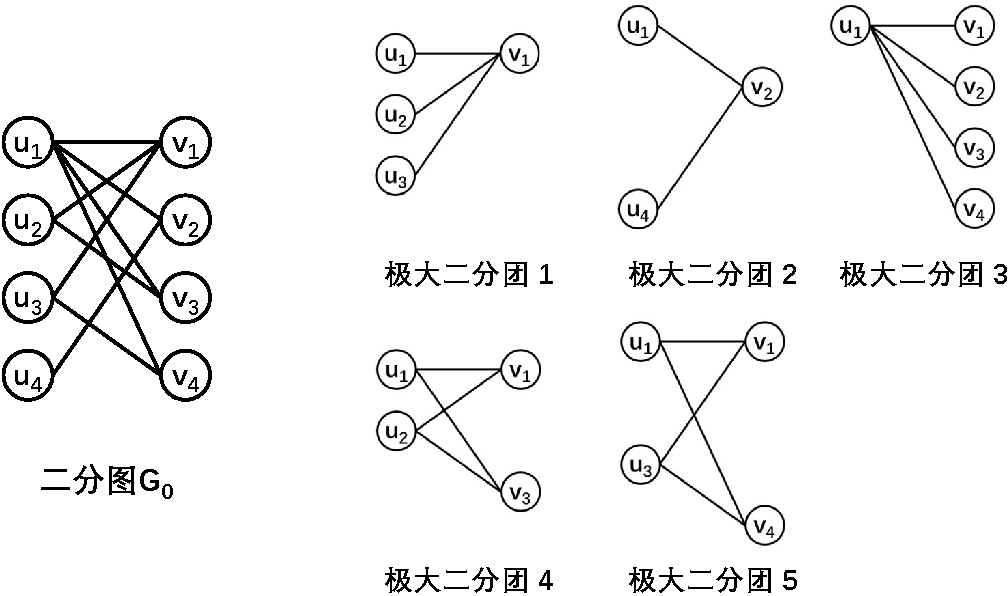
\includegraphics[width=0.7\linewidth]{eg_definition}
  \vspace{0.1 in}
  \caption{二分图中的极大二分团枚举问题示例}
  \label{fig:eg_definition}
\end{figure}

\begin{example}
  图~\ref{fig:eg_definition}给出了一个二分图中的极大二分团枚举问题的示例。其中左图是一个具有8个顶点,9条边的二分图$G_0$,右图展示了二分图中的全部极大二分团,共5个。极大二分团枚举问题即无重复、无遗漏地枚举二分图$G_0$中的全部5个极大二分团。
  
\end{example}

考虑到现有方法在处理大规模二分图时效率低下,本研究从\emph{剪枝能力} 、 \emph{数据结构} 和 \emph{并行实现}等方面入手,探索\textbf{面向大规模二分图场景的高效极大二分团枚举方法}。



% 探索在大规模二分图中高效解决极大二分团枚举问题的方法成为一项重要的研究课题。


\subsection{基本求解方法}
\label{subsec:baseline}
  
  在本节中,我们详细描述了主流的基于集合枚举树的极大二分团问题基本求解方法。我们首先介绍了极大二分团问题中的集合枚举树的定义,接着给出了基于该集合枚举树的极大二分团枚举基本算法,最后分析了该算法的复杂度。

\subsubsection{集合枚举树介绍}
\label{subsec:se}

\begin{figure} [ht]
  % \vspace{0.1 in}
  \centering
  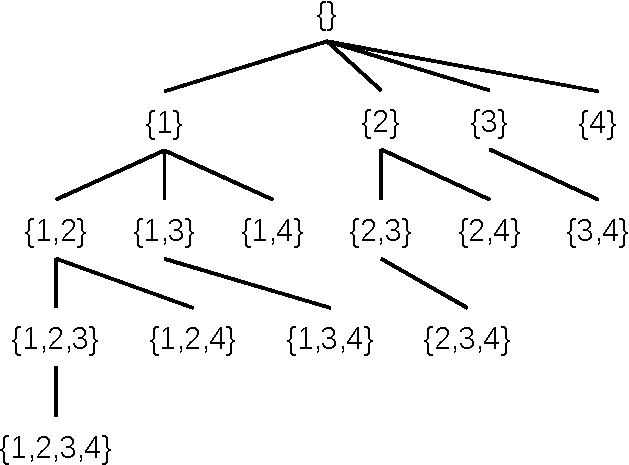
\includegraphics[width=0.45\linewidth]{se_naive}
  \vspace{0.1 in}
  \caption{对于集合$P\{1,2,3,4\}$的集合枚举树}
  \label{fig:se_naive}
\end{figure}


\textbf{集合枚举树}(Set Enumeration Tree, SE tree)是一种用于有序地枚举特定集合全部子集的数据结构,即枚举该集合的幂集~\cite{SEtree92}。它为解决搜索空间为特定集合幂集的子集的问题提供了一种完整且无冗余的搜索技术。具体而言,集合枚举树如图~\ref{fig:se_naive} 所示,根节点表示空集,每个节点对应一个子集,其子节点代表在该子集基础上添加一个新元素所得到的子集。对于二分图中的极大二分团枚举问题而言,每个二分团的集合$R$即为二分图中集合$V$的一个独特子集。因此,通过引入集合枚举树可以无重复、无遗漏地枚举全部可能的极大二分团,进而有效地求解极大二分团枚举问题。

对于应用于极大二分团枚举问题的集合枚举树,我们从以下三个角度对其进行了规范化描述:

\begin{itemize}
  \item 节点结构:每个树节点为一个三元组$(L,R,C)$。在一个二分图$G(U,V,E)$,集合$L$是集合$U$的子集,集合$R$和集合$C$是集合$V$的两个不相交子集。集合$L$和$R$构成一个二分团,其中集合$L$包含左部顶点,集合$R$包含右部顶点。集合$C$包含用于扩展集合$R$的候选顶点。
  \item 节点生成:枚举树从根节点$(U,\emptyset,V)$ 开始遍历。对于当前节点$(L,R,C)$,枚举树按顺序访问集合$C$中的每个候选顶点$v'$以生成一个新的节点$(L',R',C')$。集合$L'$包含集合$L$和集合$N(v')$中的共同顶点。集合$R'$包含集合$R$中的顶点、顶点$v'$以及集合$C$中与集合$L'$内顶点均相连且未被访问的顶点。集合$C'$包含集合$C$中与集合$L'$内顶点部分相连的且未被访问的顶点。
  \item 节点检查:当且仅当集合$L'$的共同邻居等于集合$R'$, 即$\Gamma(L')=R'$时,节点$(L',R',C')$通过节点检查,输出一个极大二分团。
\end{itemize}

此外,一些研究~\cite{iMBEA14,ooMBE22}在每个枚举节点中额外引入集合$Q$作为辅助节点检查的工具,构成四元组$(L,R,C,Q)$。其中集合$Q$于存储已访问的候选顶点,以帮助检查节点是否对应非极大二分团。具体而言,当集合$Q$中存在任意一个顶点$v_q$,并且它的邻居包含了集合$L$中的所有顶点时,根据定义~\ref{def:mb}我们可以推断当前节点对应的二分团$(L,R)$可以添加顶点$v_q$构成新的二分团,即$(L, R\cup\{v_q\})$,从而我们可以判定当前节点对应一个非极大二分团。然而,使用集合$Q$需要额外的存储和计算开销。幸运的是,我们观察到可以通过访问$L$中的任意顶点$u_l$的邻居$N(u_l)$来高效地替代集合$Q$的作用。具体而言,当集合$N(u_l)$中存在一个不在$R$集合中的顶点$v^*$,并且它的邻居包含了集合$L$中的所有顶点时,我们可以推断当前节点对应的二分团$(L,R)$可以添加顶点$v^*$构成新的二分团,从而判定当前节点对应一个非极大二分团。因此,在枚举树的介绍和相关算法中,我们不再引入集合$Q$。

\subsubsection{基于集合枚举树的极大二分团枚举基本算法}
\label{subsec:algorithm}
  结合上一节对集合枚举树的定义与描述,我们给出了基于集合枚举树的极大二分团枚举基本算法。

\begin{algorithm}[H]
    \begin{algorithmic}[1]
        \normalsize
        \REQUIRE 二分图 $G(U,V,E)$
        \ENSURE 所有极大二分团
        
        \renewcommand{\algorithmicwhile}{\textbf{procedure}}
        \renewcommand{\algorithmicdo}{\textbf{:}}


        \STATE \textsf{biclique\_search\_basic}$(U,\emptyset,V)$;
        \WHILE{\textsf{biclique\_search\_basic}$(L,R,C)$}
        \renewcommand{\algorithmicdo}{\textbf{do}}
          \FOR{$v' \in C$}
            \STATE $L' \leftarrow L \cap N(v')$; $R'\leftarrow R$; $C' \leftarrow \emptyset$;
            \FOR{$v_c \in C$}
              \IF{$L' \cap N(v_c) = L'$}
                \STATE $R' \leftarrow R' \cup \{v_c\}$;
              \ELSIF{$L' \cap N(v_c) \neq \emptyset$}
                \STATE $C' \leftarrow C' \cup \{v_c\}$;
              \ENDIF
            \ENDFOR
            \IF{$\Gamma(L') = R'$}
              \STATE 输出极大二分团$(L', R')$;
              \STATE \textsf{biclique\_search\_basic}$(L',R',C')$;
            \ENDIF
            \STATE $C \leftarrow C \setminus \{v'\}; $
          \ENDFOR

        \ENDWHILE

    \end{algorithmic}
    \caption{基于集合枚举树的极大二分团枚举算法}
    \label{alg:se_mbe}
\end{algorithm}

算法~\ref{alg:se_mbe}总结了基于集合枚举树的极大二分团枚举算法的基本枚举过程。具体而言,该算法从根节点$(U,\emptyset,V)$开始,递归地调用\textsf{biclique\_search\_basic}过程 (第1行)。过程\textsf{biclique\_search\_basic}接收一个枚举树节点作为输入,即该节点对应的集合$L$,$R$和$C$ (第2行)。在处理当前枚举节点时,该过程会逐个遍历$C$中的顶点$v'$ (第3行),然后根据集合枚举树的节点生成规则生成新节点$(L',R',C')$ (第4-11行)。随后,过程按照节点检查规则对新生成的节点$(L',R',C')$进行检查 (第12行)。如果该节点对应一个极大二分团,则输出该二分团 (第13行),并递归地调用过程\textsf{biclique\_search\_basic}以节点$(L',R',C')$为根节点继续探索子枚举树 (第14行);否则,我们知道该节点对应非极大二分团,跳过该节点。为保证$C$中的顶点都未被访问,过程会及时从$C$中移除已访问的顶点$v'$ (第16行)。我们用下面的例子对该算法进行说明。


\begin{figure} [ht]
  \vspace{0.1 in}
  \centering
  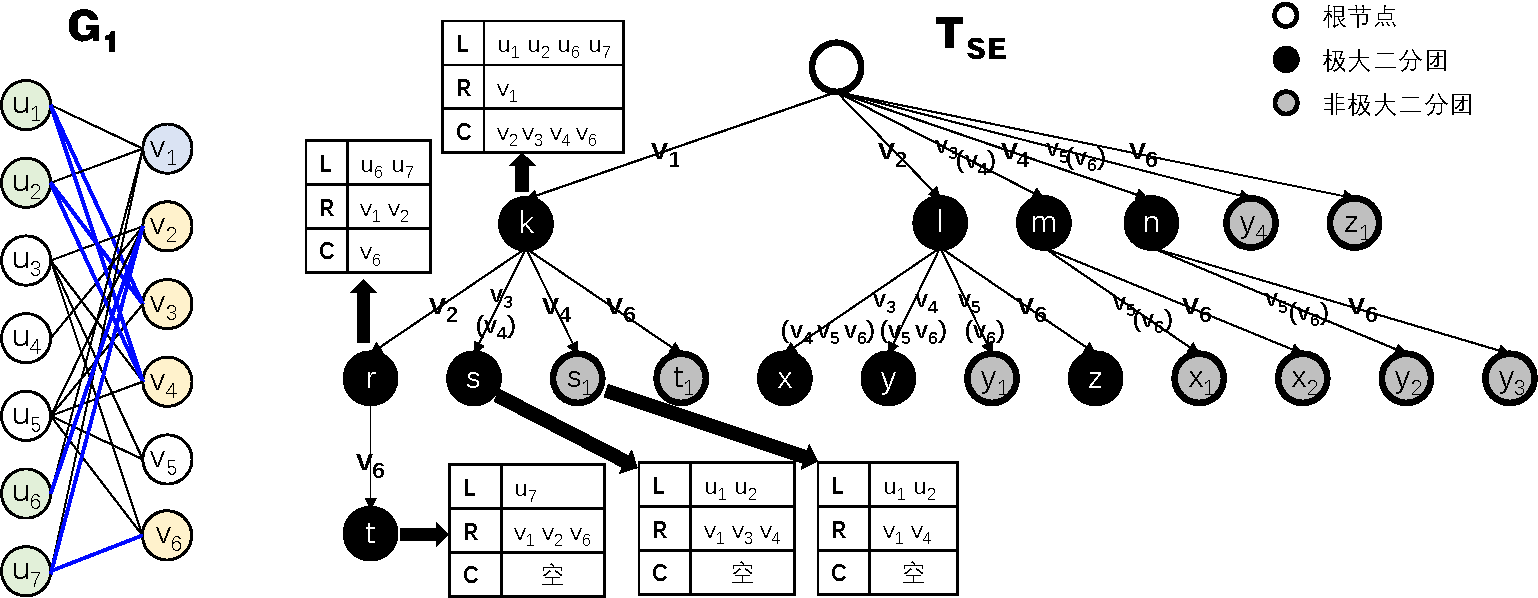
\includegraphics[width=0.98\linewidth]{se_mbea}
  \vspace{0.1 in}
  \caption{算法~\ref{alg:se_mbe}在二分图$G_1$上的集合枚举树}
  \label{fig:se_mbea}
\end{figure}

\begin{example}
  \label{example:se}
  图~\ref{fig:se_mbea}展示了算法~\ref{alg:se_mbe}在二分图$G_1$上的集合枚举树$T_{SE}$。
  \footnote{为了方便比较,全文中具有相同字母标识的节点在枚举树中共享相同的集合$L$,只有没有下标的节点会输出极大二分团。例如,节点$s$和节点$s_1$具有相同的集合$L$,但只有节点$s$会输出一个极大二分团。我们使用集合的下标来表示该集合隶属于哪个节点。例如$L_s$表示节点$s$的集合$L$。 
}
我们从根节点开始,通过深度优先搜索逐个遍历候选顶点,递归地搜索子空间。首先,我们通过遍历顶点$v_1$生成节点$k$。按照算法~\ref{alg:se_mbe}中第4-11行的计算方法,我们可以计算得到$L_k=N(v_1)=\{u_1, u_2, u_6, u_7\}$,$R_k=\{v_1\}$,$C_k=\{v_2,v_3,v_4,v_6\}$。根据节点检查规则,因为$\Gamma(L_{k}) = \{v_1\} = R_{k}$,所以节点$k$输出一个极大二分团并继续探索以节点$k$为根节点的子枚举树。为便于观察,我们在图$G_1$中标记了节点$k$中的顶点,即$L_k$,$R_k$和$C_k$中的全部顶点,并标出了集合$L_k$与集合$C_k$之间的边。

接下来,节点$k$遍历顶点$v_2$生成节点$r$。同理,我们可以计算得到$L_{r} = N(v_2) \cap L_{k} 
= \{u_3, u_4, u_5, u_6, u_7\} \cap \{u_1, u_2, u_6, u_7\} = \{u_6, u_7\}$, $R_{r} = R_{k} \cup (C_{k} \cap \Gamma(L_{r})) = \{v_1\} \cup (\{v_2, v_3, v_4, v_5\} \cap \{v_1, v_2\}) = \{v_1, v_2\}$。集合$C_{r}$中仅包含顶点 $v_6$,因为顶点$v_3$, $v_4$和 $v_5$不与集合$L$中的任何顶点相连。

继续这个过程,我们可以计算得到节点$s$以及节点$s_1$。节点$s$对应二分团$(\{u_1, u_2\},$ $\{v_1, v_3, v_4\})$,节点$s_1$对应二分团 $(\{u_1, u_2\}, \{v_1, v_4\})$。根据节点检查规则,因为$\Gamma(L_{s_1}) = \{v_1, v_3, v_4\} \neq R_{s_1} = \{v_1, v_4\}$,所以节点$s_1$对应一个非极大二分团。具体地,与节点$s$相比,节点$s_1$不能用$v_3$来扩展该节点中的集合$R_{s_1}$。这是因为在生成节点$s_1$时,根据深度优先搜索的规则,顶点$v_3$已被访问并用于生成节点$s$。因此,在节点检查之后,我们删除了节点$s_1$。同理,其他节点可以类似地生成。

\end{example}

在算法~\ref{alg:se_mbe}的基础上,现有的基于枚举树的极大二分团枚举算法的优化方法主要包括改变节点候选顶点的遍历顺序~\cite{minel06,iMBEA14,PMBE20,ooMBE22}、设计剪枝方法以提前裁剪产生非极大二分团的节点~\cite{iMBEA14,PMBE20,ooMBE22},以及并行优化~\cite{mapreduceMBE16,parMBE19}。在~\ref{sec:opt}节中,我们将对上述优化方法进行详细说明,并介绍它们在实际应用中的效果。

\subsubsection{算法复杂度分析}
\label{subsec:baseline_analysis}

结合算法伪代码,我们从时间复杂度和空间复杂度两个方面对算法~\ref{alg:se_mbe}进行分析。

\textbf{时间复杂度:} 我们首先分析枚举树中每个节点的计算时间,随后分析枚举树中的枚举节点数量,最终得到算法~\ref{alg:se_mbe}的时间复杂度。平均而言,对于每个节点$(L',R',C')$的计算包括节点生成(第4-11行)和节点检查(第12行)两个部分。由于集合$C$中最多包含$|V|$个顶点,且每个顶点的集合交集运算需要$O(\Delta(V))$的时间,因此节点生成过程的时间复杂度为$O(|V|\Delta(V))$。而节点检查过程中,我们可以通过只访问二分图中的每条边一次来获取$\Gamma(L')$的值,因此节点检查的时间复杂度为$O(|E|)$(或$O(|V|\Delta_{avg}(V))$)。综上,每个节点的计算时间为$O(|V|\Delta(V))$。为了量化算法的计算时间,我们用$\beta$来表示枚举树中节点的数量。最终,算法的时间复杂度为$O(|V|\Delta(V)\beta)$。

\textbf{空间复杂度:} 由于算法~\ref{alg:se_mbe}按照深度优先的方式进行搜索,我们可以对枚举树中每个节点占用的空间进行分析,并结合枚举树的高度以及输入二分图所占用的空间,得到算法的空间复杂度。对于每个节点$(L',R',C')$,集合$L'$最多包含$\Delta(V)$个顶点,集合$R'$和$C'$最多包含$|V|$个顶点。在二分图中,集合$V$内顶点的数量通常远高于任何单个顶点的度数,因此每个节点的空间开销为$O(\Delta(V)+|V|)=O(|V|)$。在递归过程中,节点的集合$L$内的顶点数量不断减少,因此我们可以确定枚举树的高度为$O(\Delta(V))$。考虑到二分图$G(U,V,E)$需要占用$O(|U|+|V|+|E|)=O(|E|)$的空间,最终算法的空间复杂度为$O(|E|+|V|\Delta(V))$。

